
% JuliaCon proceedings template
\documentclass{juliacon}
\setcounter{page}{1}

\usepackage{subfigure}
\usepackage{amsmath}
\usepackage{amssymb}
\usepackage{pifont}
\newcommand{\cmark}{\ding{51}}%
\newcommand{\xmark}{\ding{55}}%

\begin{document}

% **************GENERATED FILE, DO NOT EDIT**************

\title{DistributedWorkflows.jl - A Julia interface to a task-based workflow management system.}

\author[1, 2]{Firoozeh Dastur}
\author[3]{Max Zeyen}
\author[2]{Mirko Rahn}
\affil[1]{RPTU Kaiserslautern}
\affil[2]{Fraunhofer ITWM}
\affil[3]{NorthStar Earth \& Space}

\keywords{Distributed workflows, Parallel computing, Task-based computing, Petri net workflows, High-Performance Computing (HPC), User experience (UX), User-centered design (UCD)}

\hypersetup{
pdftitle = {DistributedWorkflows.jl - A Julia interface to a task-based workflow management system.},
pdfsubject = {JuliaCon 2019 Proceedings},
pdfauthor = {Firoozeh Dastur, Max Zeyen, Mirko Rahn},
pdfkeywords = {Distributed workflows, Parallel computing, Task-based computing, Petri net workflows, High-Performance Computing (HPC), User experience (UX), User-centered design (UCD)},
}



\maketitle


\begin{abstract}
\emph{DistributedWorkflows.jl} is a serializer-independent interface to a distributed task-based workflow management system.
This package aims to simplify the process of writing distributed applications.
Given a workflow pattern in the form of a Petri net and the Julia code for the workflow tasks, it can be used on a cluster, for example with Slurm, to automate the application's parallel deployment. 
This makes \emph{DistributedWorkflows.jl} an invaluable addition to Julia's growing ecosystem of high-performance computing.
\end{abstract}


\section{Introduction}
\label{sec:introduction}

Distributed computing is an essential research component and has led to significant advancements across many scientific domains.
The availability and increasing performance of HPC systems enables the realization of experiments that are too costly, too dangerous, practically infeasible, or all of the above.
Additionally, increasing data sizes and problem complexity have raised the necessity of adapting to a parallel world for many researchers.\vskip 6pt

For example, in the modeling and analysis of protein synthesis and DNA mutation, distributed systems enable efficient simulations of complex biological processes, providing insights into genetics and molecular biology (e.g. \cite{biology_example_petrinets_openaccess}).
Similarly, weather simulations have greatly benefited from distributed systems, allowing for more accurate and faster predictions (e.g. \cite{WeatherForcast_HPC_paper}).
Additionally, climate simulations are enabled to run over larger time ranges (e.g. \cite{TheJuly2019EuropeanHeatWaveinaWarmerClimateStorylineScenarioswithaCoupledModelUsingSpectralNudging}).
Other examples include asteroid impact simulations\cite{asteroid_vis_paper}, black hole mergers\cite{blackhole_merger}, and nuclear fusion simulations\cite{in_situ_visualization_large_scale_fusion_simulation}, just to name a few (see Figure \ref{fig:intro_examples}).
These achievements highlight the transformative power of distributed systems in scientific research.\vskip 6pt

However, programming distributed applications is a challenge of its own, especially for scientists who are not trained in the proper usage of HPC systems.
Although this task is ideally outsourced to qualified computer scientists, this is not always a viable option due to many different reasons (e.g. budget).\vskip 6pt

\begin{figure}[h]
    \subfigure[]{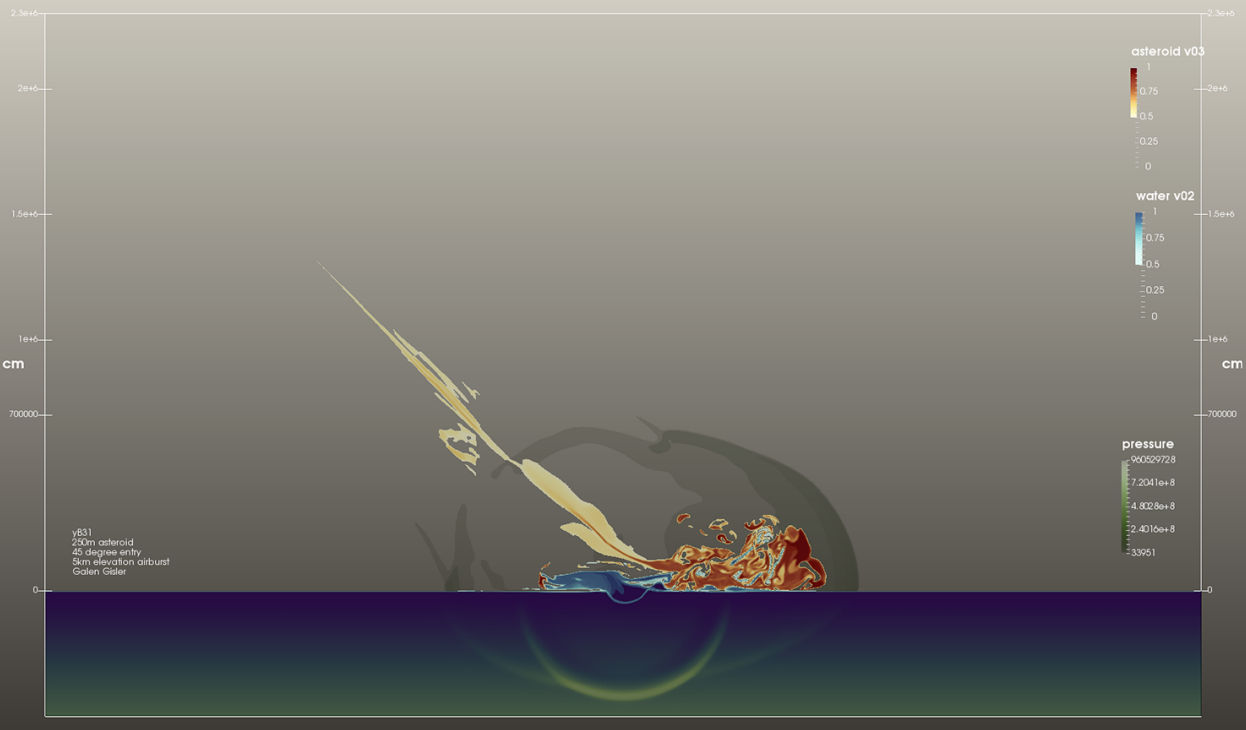
\includegraphics[width=0.5\linewidth]{asteroid-impact.png}}
    \subfigure[]{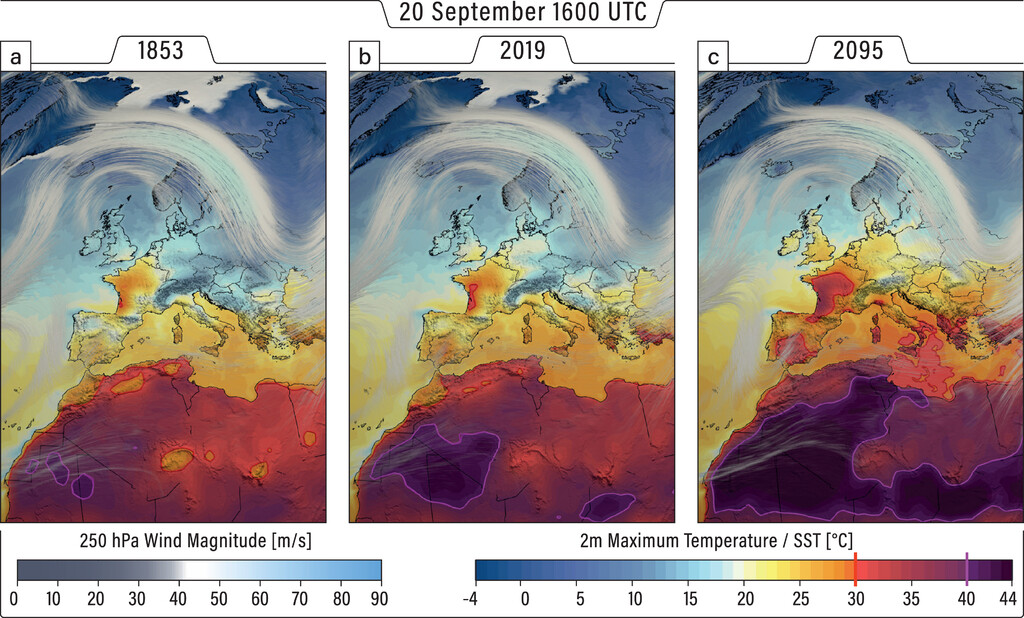
\includegraphics[width=0.5\linewidth]{climate-change.jpg}}
    \subfigure[]{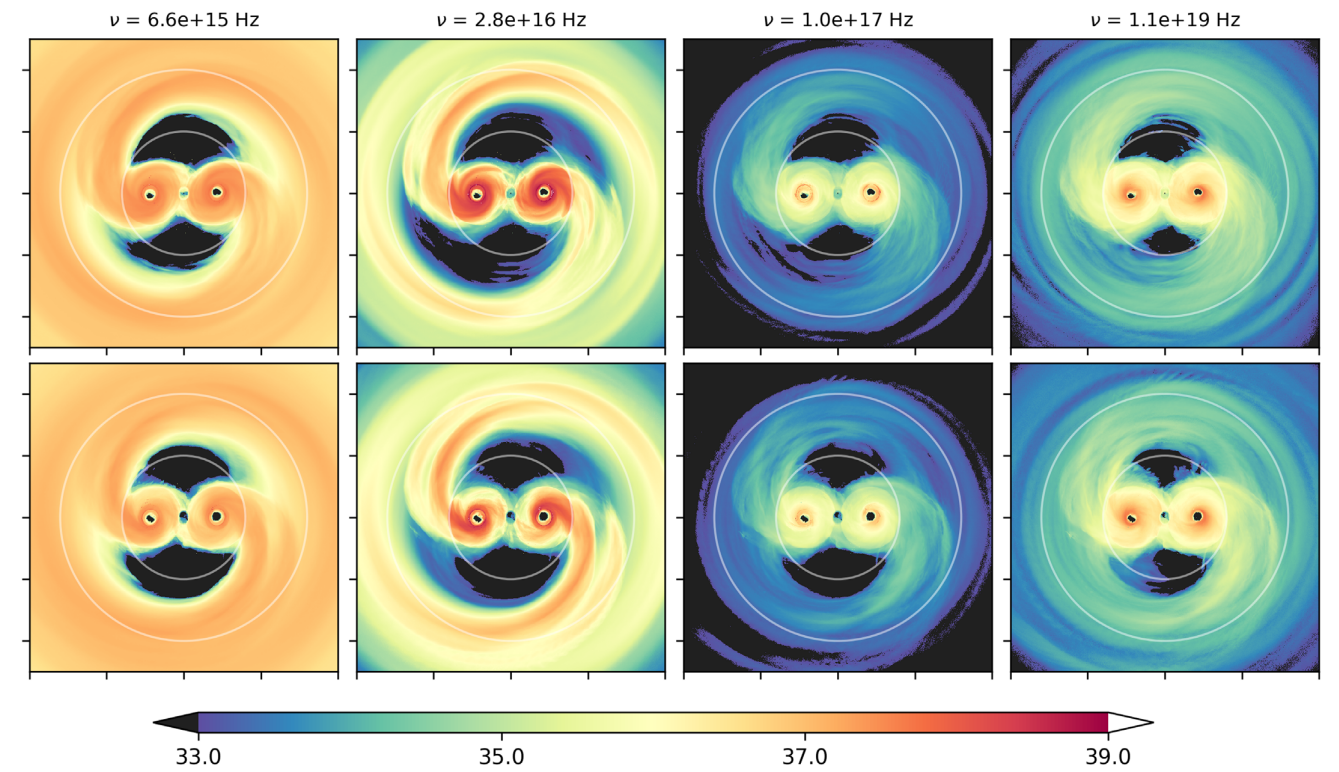
\includegraphics[width=0.5\linewidth]{black-hole-merger-02.png}}
    \subfigure[]{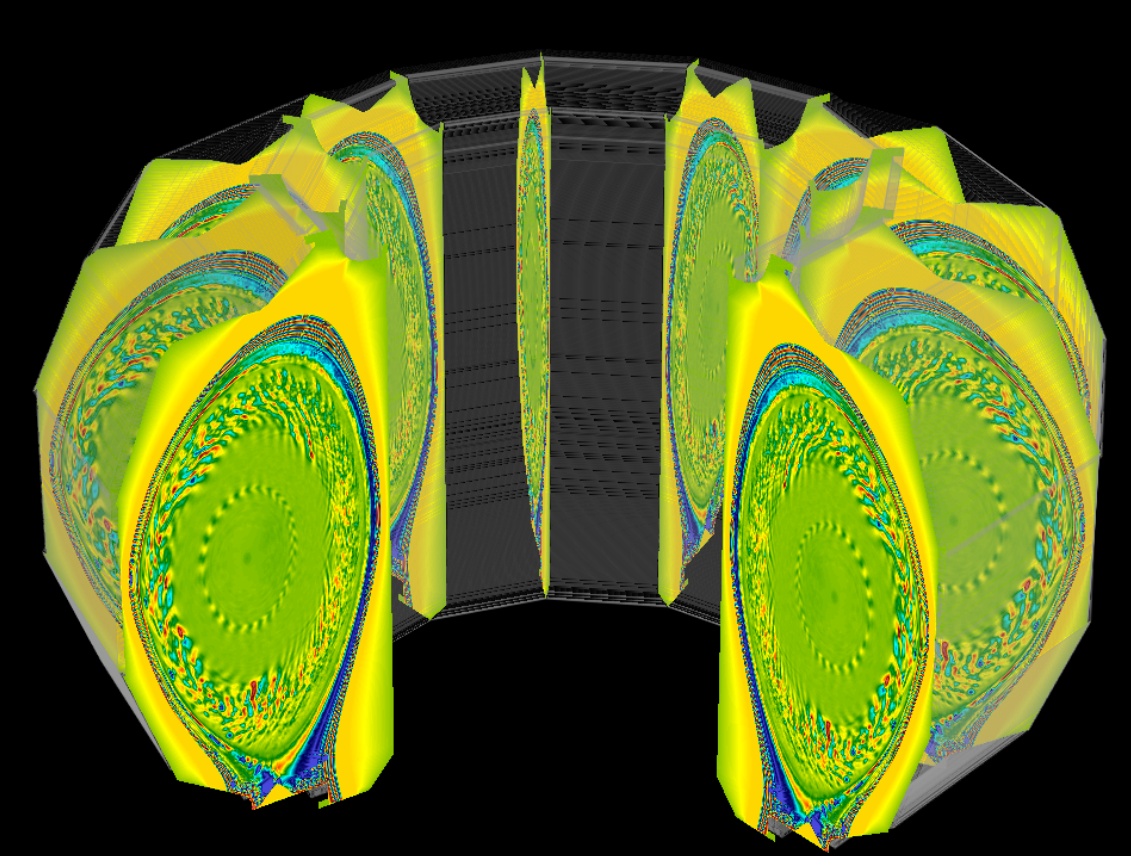
\includegraphics[height=2.5cm, width=0.5\linewidth]{nuclear-fusion-02.png}}
    \label{fig:intro_examples}
    \caption{(a) Deep ocean meteorite impact \cite{asteroid_vis_paper}, (b) evolution of future European heat waves \cite{TheJuly2019EuropeanHeatWaveinaWarmerClimateStorylineScenarioswithaCoupledModelUsingSpectralNudging}, (c) supermassive black holes merger \cite{blackhole_merger}, (d) nuclear fusion simulation \cite{in_situ_visualization_large_scale_fusion_simulation}.}
\end{figure}

Despite the clear advantages, many domain scientists struggle to write parallel applications. 
The complexity of parallel programming, coupled with the need for specialized knowledge in distributed systems, creates a barrier for scientists who are experts in their fields but not in computer science, particularly HPC models.\vskip 6pt

To address the challenges that arise due to large data sizes and application complexity, the concept of workflows has been introduced. 
Workflows provide a higher-level abstraction that simplifies the process of building parallel applications. 
By abstracting away much of the low-level complexity, workflows enable domain scientists to focus on the problem at hand rather than the intricacies of parallel programming. 
This approach significantly reduces the cognitive load required to implement distributed systems and makes parallel computing more accessible to non-computer scientists.\vskip 6pt

In this paper, we introduce \emph{DistributedWorkflows.jl}\cite{DistributedWorkflows}, a Julia package that aims to facilitate the writing of parallel applications. 
\emph{DistributedWorkflows.jl} is a high-level wrapper around the HPC tool GPI-Space\cite{GSPC}, which allows domain scientists to create efficient parallel applications with a user-friendly interface. 
This package simplifies the process of building distributed applications by providing a higher-level abstraction, enabling scientists to focus on their research rather than the challenges of parallel programming.\vskip 6pt

The paper is structured as follows:
In Section \ref{sec:related_work}, we provide an overview of related work in distributed computing with Julia and applications that utilize the underlying tool of DistributedWorkflows.
Section \ref{sec:background} presents background information on Petri nets and GPI-Space. 
In Section \ref{sec:design_and_method}, we highlight the main features of the package, and describe the design and methodology of the package.
Section \ref{sec:how_to_use} provides a short description of how to use \emph{DistributedWorkflows.jl}, while Section \ref{sec:limitations} discusses its limitations. 
Finally, Section \ref{sec:conclusions_and_future_work} briefly describes future work and our concluding remarks.


\section{Related Work}
\label{sec:related_work}

Julia's rich ecosystem already includes some packages for high-performance computing.
The most popular of these packages are \emph{Distributed.jl}\cite{Distributedjl} and \emph{Dagger.jl}\cite{dagger1, dagger2}.\vskip 6pt

\emph{Distributed.jl} offers functionalities for creating and managing multiple Julia processes remotely, enabling distributed and parallel computing. 
It utilizes network sockets or other supported interfaces to facilitate communication between Julia processes and relies on Julia’s serialization package from its standard library to efficiently transfer Julia objects between processes. 
The package includes a comprehensive set of utilities for creating and destroying Julia processes, adding them to a "cluster" (a collection of interconnected Julia processes), and enabling Remote Procedure Calls (RPC) between processes within the cluster. 
However, it requires the manual launching of tasks, which adds complexity to managing distributed workloads and makes it less user-friendly for domain scientists.\vskip 6pt

\emph{Dagger.jl} is a scheduler that draws inspiration from Dask\cite{dask}. 
It efficiently executes computations represented as directed-acyclic graphs (DAGs) across multiple Julia worker processes and threads, as well as GPUs via \emph{DaggerGPU.jl}. 
While DAGs are a powerful way to represent dependencies in a computation, as the name suggests, they cannot represent cyclic dependencies.\vskip 6pt

\emph{DistributedWorkflows.jl} uses GPI-Space\cite{GSPC} as its underlying framework.
GPI-Space has been utilized across a wide range of domains, from big-data processing \cite{gpispace_paper_mapreduce}, reverse time migration for seismic measurement data \cite{gpispace_paper_seismic}, to computational algebraic geometry \cite{gpispace_paper_singular}.
It employs Petri nets as its workflow description language, which were named after Carl Adam Petri, who extensively analyzed these graphs in his dissertation\cite{petri_nets}.
Petri nets are directed bi-partite graphs capable of modeling both concurrency and resource sharing more naturally.
In Petri nets, the transitions and places provide a richer representation of parallelism, and workflows can easily capture more complex interactions in distributed systems. 
This makes Petri nets, as used in \emph{DistributedWorkflows.jl}, a more powerful model for designing distributed applications, as they allow for greater expressiveness and ease in handling complex tasks and synchronization.
Table \ref{comparison table for distributed, dagger, and distributedworkflows} provides a feature comparison between \emph{Distributed.jl}, \emph{Dagger.jl}, and \emph{DistributedWorkflows.jl}.\vskip 6pt

This package was created out of the need to provide a convenient way to parallelize computations in the Julia package \emph{Oscar}\cite{OSCAR}. \emph{Oscar} is a computer algebra system that combines the capabilities of its four cornerstones \emph{GAP}\cite{GAP4}, \emph{Polymake}\cite{Polymake}, \emph{Antic}\cite{Antic} and \emph{Singular}\cite{DGPS_Singular}. Each of these cornerstones come equipped with their own serializer, in addition to \textsc{Oscar}'s own serializer that works from within Julia. Hence, the need of \emph{DistributedWorkflows.jl} to be serializer independent.\vskip 6pt

\emph{Singular} already employs GPI-Space to write parallel applications, for example see \cite{gpispace_paper_singular}. 
However, \emph{Singular}’s workflows are custom-designed for specific applications and are not reusable across different tasks. 
Another challenge is the need to compile the workflow Petri net along with the executable code, making it more difficult to debug and structure parallel applications. 
Although \emph{Singular} has been using GPI-Space for some time, it lacks a user-friendly interface. 
Furthermore, \emph{Singular}’s serializer is fixed to its custom \verb+ssi+ format.\vskip 6pt

In contrast, Julia’s flexibility allows users to bring their own serializer, which makes \emph{DistributedWorkflows.jl} a more versatile package in terms of serialization options.\vskip 6pt

\begin{table}[h]
\tbl{Comparison table reflecting different features of packages.}{
    \begin{tabular}{|p{7em}|c|c|c|}
        \hline
        Feature & Distributed.jl & Dagger.jl & DistributedWorkflows.jl\\
        \hline
        Low-level & \cmark & \xmark & \xmark \\
        \hline
        Task based & \xmark & \cmark & \cmark \\
        \hline
        Automated task execution & \xmark & \cmark & \cmark \\
        \hline
        Serializer independent & \xmark & \xmark & \cmark \\
        \hline
        Out of the box cyclic workflows & \xmark & \xmark & \cmark \\
        \hline
        Built-in fault tolerance & \xmark & \cmark & \cmark \\
        \hline
    \end{tabular}
    }\label{comparison table for distributed, dagger, and distributedworkflows}
\end{table}

\section{Background}
\label{sec:background}

In this section, we provide a short background on Petri nets used to define workflows in \emph{DistributedWorkflows.jl} and its underlying distributed execution framework GPI-Space.

\subsection{Petri Nets}
\label{sec:petri_nets}

The programming model of \emph{DistributedWorkflows.jl} uses Petri nets to define workflow patterns, which enable the modeling of concurrent and distributed systems.\vskip 6pt

A (basic) \emph{Petri net} $\mathcal{PN}$ is a logic model that represents the order in which the events occur. 
We define a Petri net as a bipartite graph connecting nodes "places" to "transitions" via directed graphs, see Figure \ref{basic_petri_net}. 
In other words, a Petri net can be defined mathematically as a tuple $\mathcal{PN}~:=~(P, T, F, M)$, where:
\begin{enumerate}
    \item $P$ is a finite collection of places.
    \item $T$ is a finite collection of transitions.
    \item $F$ defines the arcs or flow relations, connecting a place $p \in P$ to a transition $t \in T$ or vice versa.
    \item $M$ is the (initial) “Marking”. It is a function from $P \rightarrow N$, where $N \in \mathbb{N}$ is the number of tokens in a place.
\end{enumerate}

\begin{figure}[h]
    \centerline{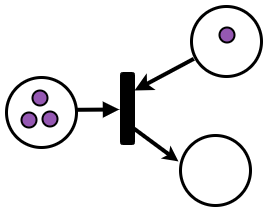
\includegraphics[width=4cm]{basic_petri_net.png}}
    \caption{A simple Petri net where the circular nodes are places, the black rectangle is a transition and the colored dots are tokens.}
    \label{basic_petri_net}
\end{figure}

Some definitions also use an additional parameter $W$ which is a weight function $W : F \longrightarrow \mathbb{N}^+$ assigning positive integers to each arc connecting places to transitions.\vskip 6pt

Petri nets have gotten multiple extensions over the years to improve their modeling convenience and/or add to their computational power.
We list a few of them below:

\begin{enumerate} 
    \item \textbf{Colored Petri nets} add data attributes (colors) to tokens, enabling easier modeling of complex systems with structured information. 
    \item \textbf{Timed Petri nets} incorporate timing constraints on transitions, making them suitable for real-time systems. 
    \item \textbf{Stochastic Petri nets} introduce probabilistic firing times, commonly used for performance and reliability analysis. 
    \item \textbf{Hierarchical Petri nets} support modularity by nesting Petri nets within others, facilitating the modeling of large-scale systems.
    \item \textbf{Continuous Petri nets} generalize tokens to real numbers and transitions to continuous dynamics, ideal for systems like fluid flow. 
    \item \textbf{Inhibitor Petri nets} include special arcs called inhibitors, which make the Petri net formalism Turing complete.
    \item \textbf{High-level Petri nets} combine features of these types, offering flexible modeling for abstract or multifaceted systems.
\end{enumerate}

\emph{DistributedWorkflows.jl} uses high-level, timed, and colored Petri nets to be consistent with GPI-Space, our underlying system.
Additionally, we support a special kind of transition called \verb+conditional transitions+ which also comes from GPI-Space. This is a special case built on top of inhibitor Petri nets.
These are required to make Petri nets non-deterministic and in turn Turing complete.
For more details on Petri nets and its applications see \cite{Introduction_to_petri_nets_book, Understanding_Petri_nets_book, IEEE_1989paper_petrinets_and_its_applications, petri_nets_paper_IEEE_inhibitor_nets}.\vskip 6pt

\subsection{GPI-Space}
\label{sec:gpispace}

GPI-Space is a task-based workflow management system for parallel applications written in C++.
It utilizes the aforementioned Petri nets to define its workflows.
Petri nets are defined using an \verb+XML+ dialect called \verb+XPNet+.
\verb+XPNet+ files are compiled into shared libraries for execution by GPI-Space applications.\vskip 6pt

The framework builds on an “agent-worker” architecture, as shown in the Figure \ref{GPISpace_arch}.
The agent houses the workflow engine and the scheduler.
The workflow engine is responsible for determining which transitions in the Petri net can be fired.
Next, exactly one token for each input place is consumed and bundled together with the transition into an activity.
Activities are handed over to the scheduler to be queued up for execution with a worker.
The worker processes that execute the tasks are distributed across the compute nodes. 
The Remote Interface Daemon (RIFD) on each host coordinates startup and shutdown steps.
The Workers and the RIFDs together constitute the Distributed Runtime System (DRTS), as depicted in Figure \ref{GPISpace_arch}.
Finally, activity results are passed back from the scheduler to the workflow engine where the outputs are put as tokens into their corresponding place.

\begin{figure}[h]
    \centerline{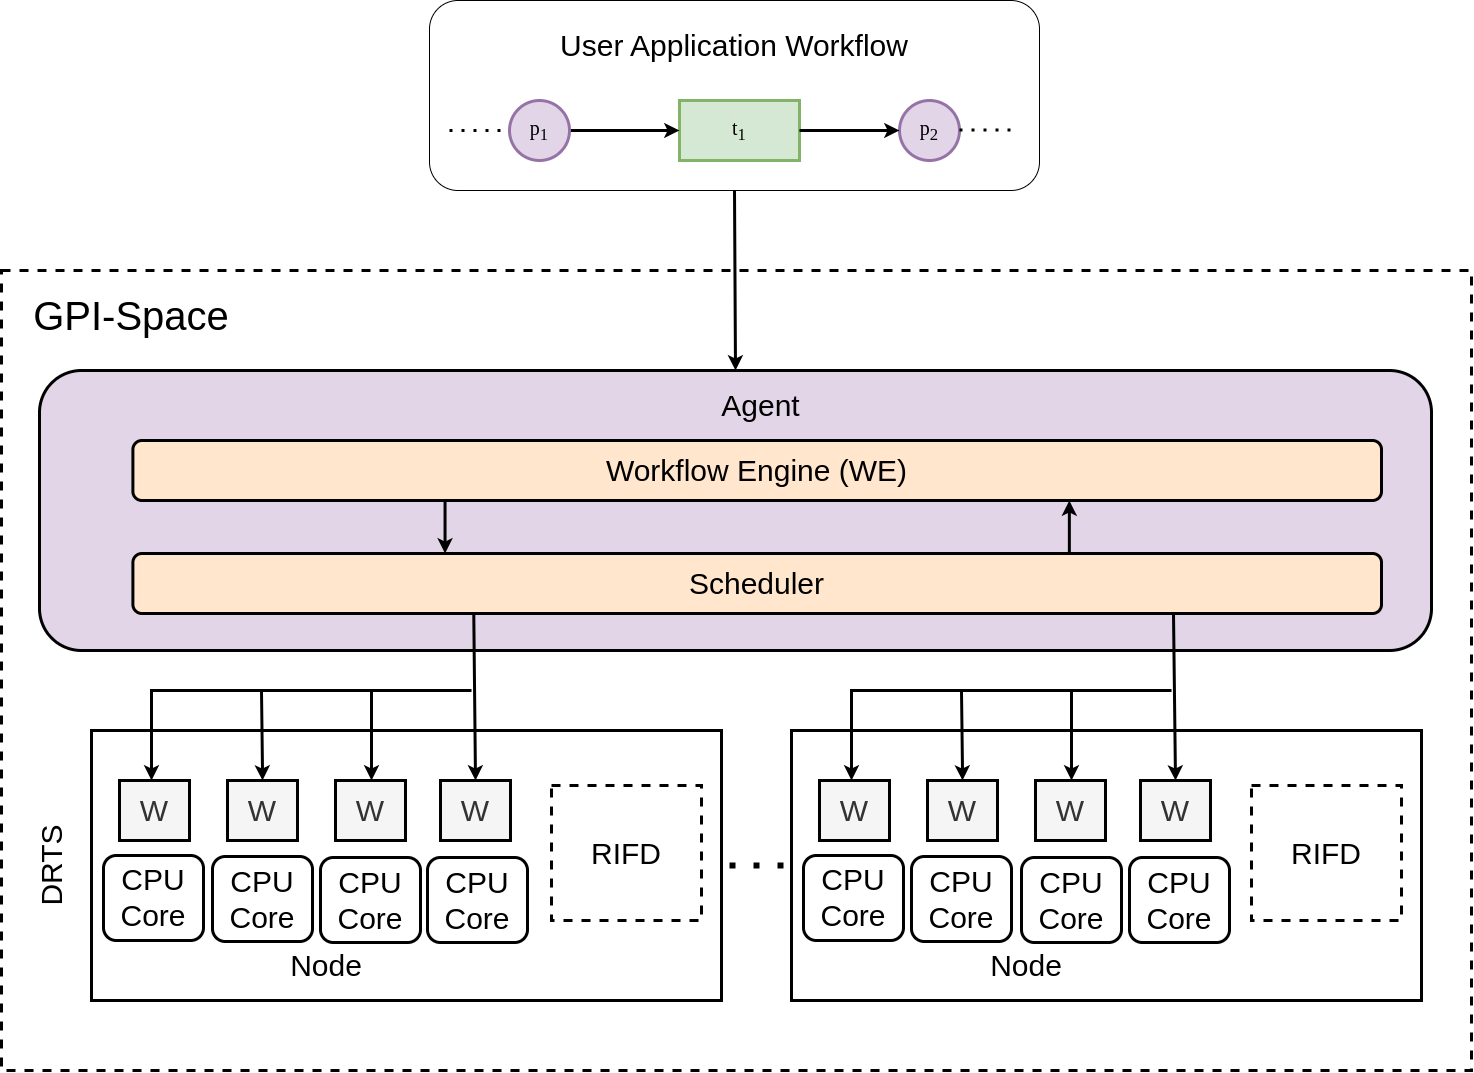
\includegraphics[width=8cm]{GPISpace_arch.png}}
    \caption{Top block shows a local portion of the user application workflow. The lower block shows how GPI-Space handles the information internally. For source image see \cite{GSPC}.}
    \label{GPISpace_arch}
\end{figure}


\section{Design and Method}
\label{sec:design_and_method}

The \emph{DistributedWorkflows.jl} package started as an interface to GPI-Space\cite{GSPC}, but it has grown to include features that significantly improves user experience.
The primary focus being on ease of use and flexibility, this package extends the capabilities of the underlying system.
Below is a summary of its key features:

\begin{itemize}
    \item \textbf{Ease of use}\\
          Designed to simplify user interactions, with a fully documented public API, consisting of examples for every method.\vskip 6pt
    \item \textbf{Serializer Independent}\\
          Supports Julia's built-in serializer, as well as other serializer formats like JLD2\cite{JLD2}, HDF5\cite{HDF5}, or any other custom serializer see for example the serializer for Julia package Oscar\cite{OSCAR}, allowing for flexibility in data handling.\vskip 6pt
    \item \textbf{Simplified Workflow Creation}\\
          Reduced complexity of writing parallel applications and the Petri net workflows, making it accessible to experts and non-experts alike.\vskip 6pt
    
    \item \textbf{Workflow Component Creation}\\
          Allows users to create Petri net workflow components without requiring a fully functional application.\vskip 6pt
    \item \textbf{Workflow Component Editing}\\
          Has the ability to add and/or remove parts of any Petri net component, giving users greater control over the workflow design.\vskip 6pt
    \item \textbf{Workflow Visualization}\\
          Features a visualization tool using Graphviz\cite{Graphviz81:online} to generate and view Petri nets, aiding in workflow design.\vskip 6pt
    \item \textbf{XML File Generation and Compilation}\\
           Includes a convenience function to generate and compile workflows into XML files required by GPI-Space, directly within Julia.\vskip 6pt
    \item \textbf{Reusable Workflows}\\
          The compiled workflows are reusable and can be applied to various applications following the same workflow pattern. 
          That is, the same workflow can be used by multiple applications by simply modifying the Julia code for the transitions in the application configuration.\vskip 6pt
    \item \textbf{Local Testing}\\
          Enables local testing of applications before deploying them on expensive cluster resources.\vskip 6pt
    \item \textbf{Easy Application Debugging}\\
          Enables easy debugging for individual transitions in the Petri net from within Julia.\vskip 6pt
    \item \textbf{Direct Job Submission}\\
          Supports job submission directly from Julia, streamlining deployment.\vskip 6pt
    \item \textbf{Notebook Support}\\
          Integrates with Jupyter\cite{Jupyter} and Pluto\cite{Plutojl} notebooks, enabling workflow viewing and editing in an interactive environment, see Figure \ref{notebook_examples}.\vskip 6pt
\end{itemize}

\begin{figure}[h]
    \centering
    \subfigure[]{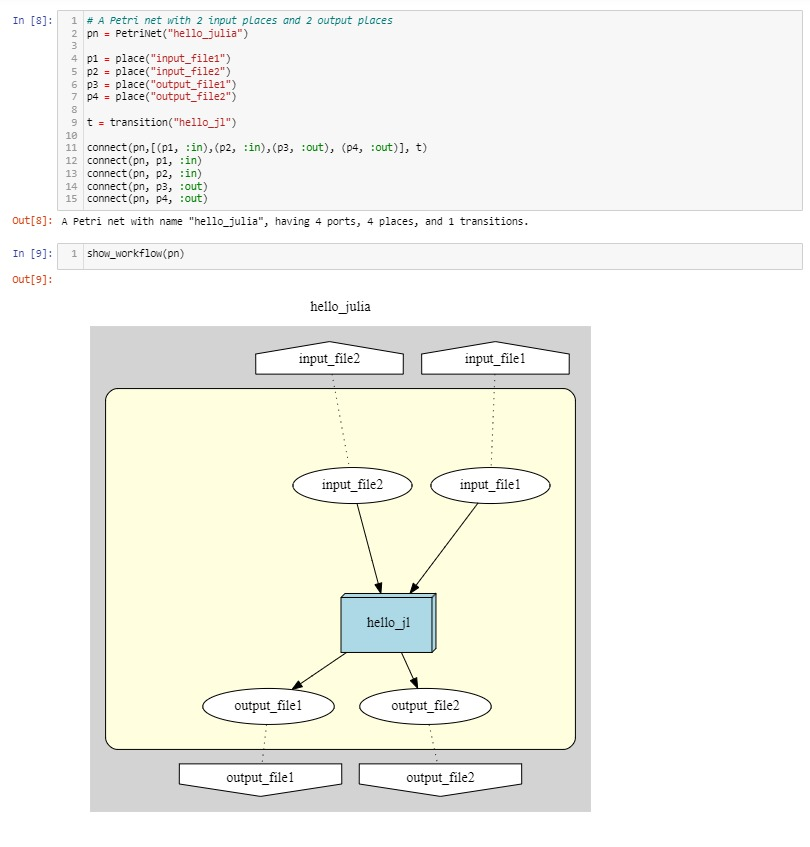
\includegraphics[height=6cm, width=\linewidth, keepaspectratio]{jupyter_example.jpeg}}
    \subfigure[]{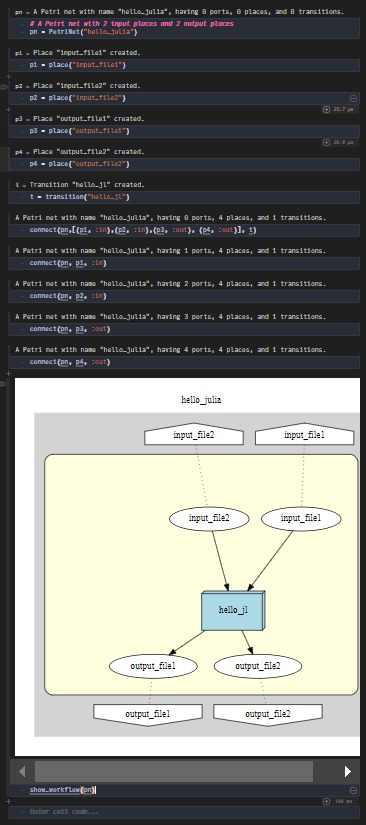
\includegraphics[height=6cm, 
 width=\linewidth, keepaspectratio]{pluto_example.jpeg}}
    \label{notebook_examples}
    \caption{Snippet of a simple Petri net workflow created and viewed using a \emph{Jupyter} notebook in (a), and a \emph{Pluto} notebook in (b).}
\end{figure}


This package has been designed with a user-centric approach from its inception.
Our primary goal has been to remove the complexities of writing parallel applications and make distributed computing more accessible to domain scientists.
As a result, users can focus on parallelizing their algorithms and designing a Petri net to define the workflow, rather than dealing with system setup intricacies. 
To achieve this, we abstracted the C++ components of GPI-Space into a library and integrated its communication functionality into Julia using CXXWrap\cite{cxxwrap}.\vskip 6pt

Since GPI-Space is a workflow management tool not natively designed for Julia, users need to configure their environment to utilize it.
GPI-Space itself can be downloaded by following the installation steps provided in \cite{GSPC}.
\emph{DistributedWorkflows.jl} on the other hand, provides binaries for selected operating systems and architectures, that can be downloaded from the GitHub repository \cite{DistributedWorkflows}.
Following the step by step instructions, the user can setup their environment to use the package.\vskip 6pt

For users who wish to visualize workflows before compilation, it is recommended to install Graphviz\cite{Graphviz81:online}, which allows visualization in various formats. 
Once the setup is complete, the \emph{DistributedWorkflows.jl} package can be installed directly in Julia using its package manager. 
At this stage, users are ready to parallelize and execute their applications with \emph{DistributedWorkflows.jl}.\vskip 6pt

Without the interface of \emph{DistributedWorkflows.jl}, the user will have to embed their parallel Julia algorithm within the workflow which is written in the \verb+XML+ based \verb+XPNet+ format. 
The workflow can only be visualized after the \verb+XML+ is compiled with functioning code.
For an example snippet see Listing \ref{lst:gspc_xpnet_example}.

\begin{lstlisting}[
    language = XML,
    captionpos = b,
    caption = \relax,
    label = {lst:gspc_xpnet_example}]
<defun name="hello_world">
  <in name="Input" place="Input" type="string"/>
  <out name="Output" place="Output" type="string"/>
  <net>
    <place name="Input" type="string"/>
    <place name="Output" type="string"/>
    <transition name="greet">
      <defun>
        <in name="Input" type="string"/>
        <out name="Output" type="string"/>
        <module name="hello_world" 
                function="greet (Input, Output)">
          <cinclude href="string"/>
          <code><![CDATA[
            Output = "Hello " + Input;
          ]]></code>
        </module>
      </defun>
      <connect-in place="Input" port="Input"/>
      <connect-out place="Output" port="Output"/>
    </transition>
  </net>
</defun>
\end{lstlisting}

The \emph{DistributedWorkflows.jl} package provides a workflow builder in the form of a Petri net, developed entirely in Julia, which can be visualized and edited without compiling the workflow or having a running code available. See for example Listing \ref{lst:distributed_workflows_pnet_example}.

\begin{lstlisting}[
    language = Julia,
    captionpos = b,
    caption = \relax,
    label = {lst:distributed_workflows_pnet_example}]
pnet = Workflow_PetriNet("hello_world")
p1 = place("Input")
p2 = place("Output")
t1 = transition("greet")
connect(pnet,[(p1,:in),(p2,:out)],t1)
connect(pnet,[(p1,:out),(p2,:in)])

# Visualizing the workflow before generating the XML file
show_workflow(pnet)
# Generating the XML file
generate_workflow(pn, "tmp/new_workflow")
\end{lstlisting}

Once the algorithm has been parallelized in the form of a Petri net workflow, users require to write a workflow launcher, compile everything, and write an executable script, in case of using GPI-Space (see GPI-Space documentation \cite{GSPC}).
We simplify the process of creating a workflow launcher and the process of compiling and executing by providing easy to use API functions in Julia.
For examples, see the examples directory in the GitHub repository \cite{DistributedWorkflows}.\vskip 6pt

Additionally, since GPI-Space is agnostic to the serializer in Julia, we provide an easy way of using any kind of serializer format, in case the user's application does not use the serializer from Julia's standard library.
See \verb+examples/other_serializers+ in \cite{DistributedWorkflows} for an example with a custom serializer.\vskip 6pt


\section{How to Use \emph{DistributedWorkflows.jl}}
\label{sec:how_to_use}

In this section, we will give a simple example showcasing the use of \emph{DistributedWorkflows.jl} for parallel applications in the Julia ecosystem.\vskip 6pt

Let us consider an example from geometry, where we want to compute the \emph{Minkowski sum} for $A_1, \ldots, A_n$, where each $A_i$ is a set of position vectors in the Euclidean space.\vskip 6pt

The \emph{Minkowski sum} of two sets of position vectors $U$ and $V$ in the Euclidean space is computed by adding each vector in $U$ to each vector in $V$, i.e. $$U + V := \{ u+v \; | \; u \in U, \; v \in V \}.$$\vskip 6pt

A Petri net describing the workflow to compute the \emph{Minkowski sum} $\sum_{i=1}^n A_i$, for $n \in \mathbb{N}$, in parallel is given in Figure~\ref{patrinet_example_how_to_use}.\vskip 6pt

\begin{figure}[h]
    \centerline{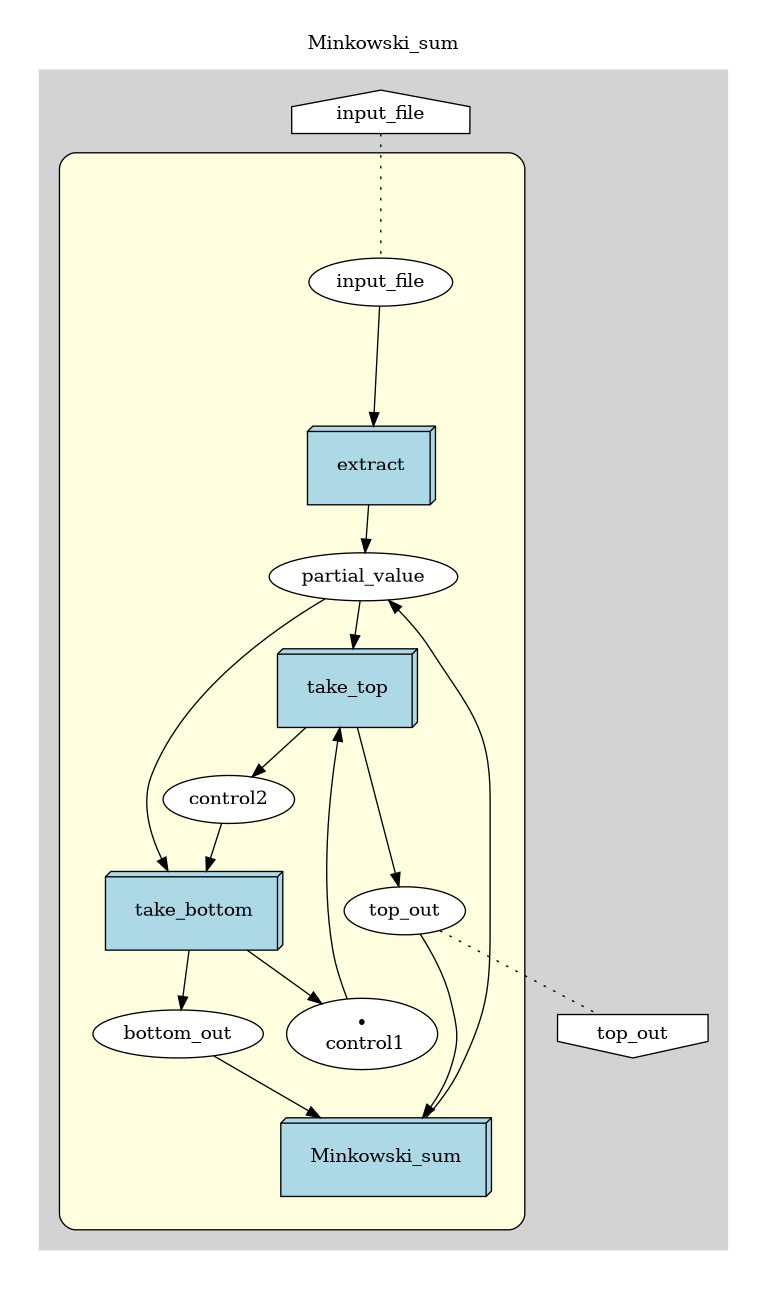
\includegraphics[height=9cm, keepaspectratio]{Minkowski_sum.png}}
    \caption{A Petri net (generated using \emph{DistributedWorkflows.jl}) modeling the workflow to compute the \emph{Minkowski sum} of a collection of sets of points in $\mathbb{R}^2$.}
    \label{patrinet_example_how_to_use}
\end{figure}

This Petri net can be written in Julia using \emph{DistributedWorkflows} as shown in Listing \ref{lst:distributed_workflows_pnet}.

\begin{lstlisting}[
    language = Julia,
    captionpos = b,
    caption = \relax,
    label = {lst:distributed_workflows_pnet}]
using DistributedWorkflows

# create an empty workflow
pnet = Workflow_PetriNet("Minkowski_sum")

# define all the places
p1 = place("input_file")
p2 = place("partial_value")
p3 = place("control1", :control_init)
p4 = place("control2", :control)
p5 = place("top_out")
p6 = place("bottom_out")

# define all the transitions
t1 = transition("extract")
t2 = transition("take_top", :exp)
t3 = transition("take_bottom", :exp)
t4 = transition("Minkowski_sum")

# connect the places to transitions with respective arcs
connect(pnet,[(p1,:in),(p2,:out)],t1)
connect(pnet,[(p2,:in),(p3,:in),(p4,:out),(p5,:out)],t2)
connect(pnet,[(p2,:in),(p3,:out),(p4,:in),(p6,:out)],t3)
connect(pnet,[(p5,:in),(p6,:in),(p2,:out)],t4)

# connect the input/output ports
connect(pnet,[(p1,:in), (p5,:out)])
\end{lstlisting}

Now, we can visualize the workflow using \verb+show_workflow()+ or it can be saved using a preferred format using \verb+savefig()+ methods, see Figure~\ref{patrinet_example_how_to_use}.
Once we have a satisfactory workflow, an XML file can be generated using \verb+generate_workflow()+ and later compiled using \verb+compile_workflow()+ methods.\vskip 6pt

Assuming that we have a method called \verb+Minkowski_sum(A, B)+, where the method takes as input two sets $A$ and $B$ and returns a set $C$ which is the \emph{Minkowski sum} of the input sets.
Next, we set up our workflow launcher by configuring our application as well as the workflow as shown in Listing \ref{lst:distributed_workflows_configure}.

\begin{lstlisting}[
    language = Julia,
    captionpos = b,
    caption = \relax,
    label = {lst:distributed_workflows_configure}]
# name of the input port from where the 
# serialized data enters the workflow
impl_port = "implementation_1"

jl_impl = "/path/to/code/per/transition.jl"

# name of functions corresponding to each transition
fname0 = "extract"
fname1 = "Minkowski_sum"

# configure the application
app = application_config(impl_port, 
                         jl_impl, 
                         [fname0, fname1])
out_dir = "path/to/output"

# workflow configuration 
workflow_cfg = workflow_config("Minkowski_sum.pnet", 
                                out_dir, app)

# set the input parameter for the initial state
input_stream = input_pair("input_file", 
                          "/path/to/serialized_data")

input_var = [input_stream]
\end{lstlisting}

Note, this can be saved as a Julia script to execute together with our compilation step.\vskip 6 pt

At this stage, if we are happy with the workflow and our transition code, we can compile and locally execute the application to test it, before using expensive cluster resources, as shown in Listing \ref{lst:distributed_workflows_call_workflow}.

\begin{lstlisting}[
    language = Julia,
    captionpos = b,
    caption = \relax,
    label = {lst:distributed_workflows_call_workflow}]
resource_list = joinpath(tmp_dir, "nodefile")
# start the client locally with the number of workers 
# based on the available resources.
client = client(4, resource_list , "local")

# submit the workflow to the client with 
# the workflow configuration
submit_app = submit_workflow(client, workflow_cfg, input_var)
\end{lstlisting}

Finally, depending on the cluster settings, we can run this example on a cluster. 
Note that since clusters are not standardized, the cluster execution script may vary depending on the cluster manager. 
For details on cluster managers in Julia see \cite{JuliaClusterManagers}.\vskip 6pt

As a more complex example, a Petri net workflow (see Figure \ref{complex_example}) that models different repair synthesis pathways of DNA as in \cite{biology_example_petrinets_openaccess} can also be tested using \emph{DistributedWorkflows.jl}.
In this case, since the application setup has been simplified due to the Julia interface, the most complex part will be to have the transition code in Julia that would be executed using a given workflow pattern.

\begin{figure}[h]
    \centerline{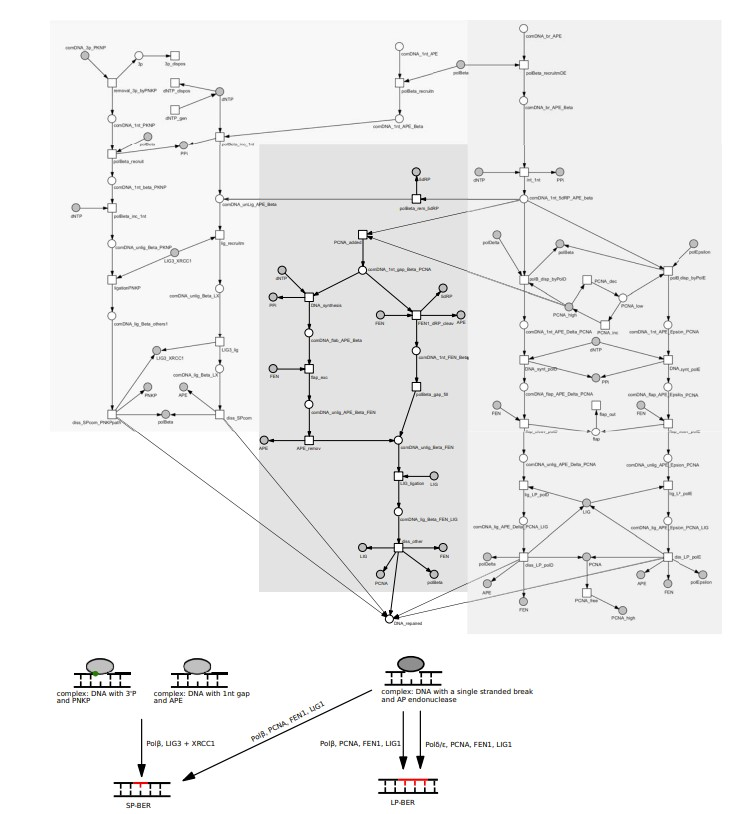
\includegraphics[width=8cm]{example_proceedings2.jpg}}
    \caption{Part of a Petri net modeling different repair synthesis pathways of DNA as in \cite{biology_example_petrinets_openaccess}.}
    \label{complex_example}
\end{figure}


\section{Limitations}
\label{sec:limitations}

Like any software, the \emph{DistributedWorkflows.jl} package has certain limitations.
It is an interface package and hence relies on tools outside of Julia.
It has somewhat of a setup process before being able to parallelize applications.
It is currently, recommended for long-running processes due to I/O overhead and requires a shared filesystem.
Official support for the workflow manager is limited to Ubuntu 20 and 22 LTS, with compatibility restricted to Linux distributions, excluding macOS and Windows.
Additionally, the package relies on Spack for binary installation, which may introduce additional setup complexity for some systems.


\section{Conclusions and Future Work}
\label{sec:conclusions_and_future_work}

This paper and the \emph{DistributedWorkflows.jl} package introduce a user-friendly interface for managing distributed, task-based workflows. 
It enables users to generate, visualize, compile, and launch workflows represented as Petri nets through simple methods. 
The package provides a fully documented public API, allowing users to locally test applications before deploying them on expensive clusters, ensuring cost efficiency. 
With binaries available for multiple Linux distributions, the tool is currently best suited for long-running processes.\vskip 6pt

Upcoming updates aim to enhance the package with specialized transition types for reduced boilerplate code, additional workflow examples to guide users, and convenience functions that streamline the process of creating and managing workflows. 
Furthermore, improvements to the user interface are planned, making the tool even more intuitive. 
These features are expected to expand the package's utility, enabling broader adoption and more efficient handling of distributed workflows across various applications.


\section{ACKNOWLEDGEMENTS}
\label{sec:acknowledgements}

We extend our gratitude to Fraunhofer ITWM for funding the Ph.D. studies of the first author. 
As well as, enabling her to work on and develop \emph{DistributedWorkflows.jl}. 
We are also deeply grateful to Prof. Dr. Anne Fr\"uhbis-Kr\"uger and Prof. Dr. Claus Fieker for their invaluable insights into the needs of domain scientists, which guided the design of this package with a strong focus on user experience. 
Our sincere thanks goes to Dr. Tiberiu Rotaru for his expertise in GPI-Space, particularly during the initial stages of integrating our Julia prototype with C++.

% **************GENERATED FILE, DO NOT EDIT**************

\bibliographystyle{juliacon}
\bibliography{ref.bib}


\end{document}

% Inspired by the International Journal of Computer Applications template
